\section{Localisation}

The study area is located bordering the Atlantic Ocean and is part of the over $27 \, 000 \, \textrm{km}^2$ extending Souss-Massa Basin in south-western Morocco (Figure \ref{Map-SoussMassaRegion}). 
The Souss-Massa Basin comprises the watersheds of the rivers Souss in the north and north-east and Massa in the south. 
The former originates in the mountains of the High Atlas to the north, the Siroua Massif to the east and the Anti Atlas to the south-east, and the latter in the Anti Atlas to the east and south-east. 
These mountains and their foothills constitute the boundaries of the basin to the north, east and south-east, while the Atlantic Ocean forms its boundary to the west. 
Below $700 \, \textrm{m.a.s.l.}$ and down to $0 \, \textrm{m.a.s.l.}$ the triangular-shaped, extensively agriculturally developed Souss plain lies embedded between the mountains and has an area of $5 \, 700 \, \textrm{km}^2$ \parencite{Choukr.2017}.
    
In this study, a model for the Chtouka aquifer is examined. 
The Chtouka aquifer underlies the agriculturally important Chtouka plain. 
It is localised within the Souss-Massa plain near the western coast, and has an area of $1 \, 300 \, \textrm{km}^2$ (Figure \ref{Map-SoussMassaRegion}). 
The Chtouka plain ranges approximately from $0 \, \textrm{m.a.s.l.}$ on the western Atlantic coast up to $348 \, \textrm{m.a.s.l.}$ in the south-eastern mountainous area. 
Sloping from east to west, $80 \, \%$ of its surface is between $50$ and $175 \, \textrm{m.a.s.l.}$.

\begin{figure}[p]
    \centering
    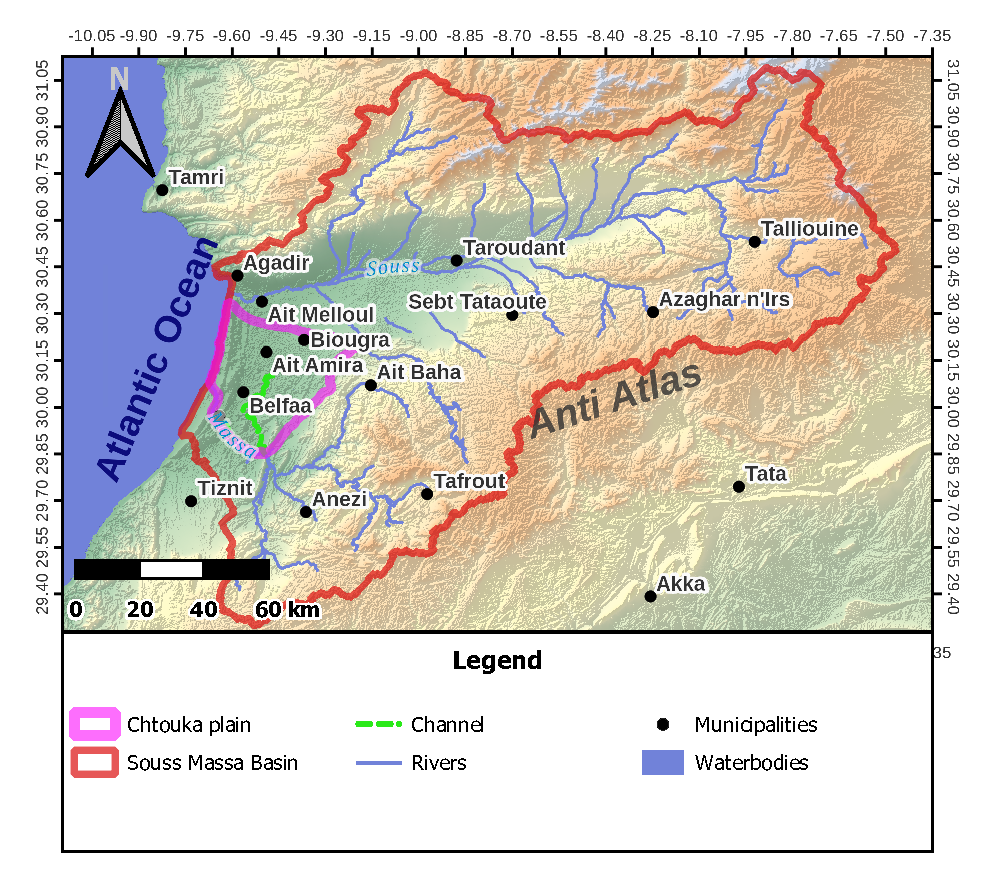
\includegraphics[width=1.0\textwidth]{./img/Map_SoussMassa.pdf}
    \caption{Map of the Souss-Massa Basin, showing the location the Chtouka plain. This representation is derived from digital elevation model data of \textcite{NASA.SRTM1Arc} and follows in topographical colouring \textcite{Hssaisoune.2017}. The small bottom-right map shows the location within Morocco.}
    \label{Map-SoussMassaRegion}
\end{figure}

\section{Geology}
\label{Sec-SouMaGeology}

The Souss-Massa plain has been formed by the homonymous rivers and their tributaries and is covered by their alluvial deposits \parencite{Hssaisoune.2017}. 
These alluvial deposits are porous and constitute an aquifer. 
The Chtouka aquifer can be characterised by four different major Plio-Quaternary geological formations according to \textcite{Malki.2017}: 
    \begin{itemize}
        \item[(i)] in the southern and eastern parts of the plain marls and limestones basing directly on Acadian age schist, 
        \item[(ii)] conglomeratic deposits in the beds of the Massa, 
        \item[(iii)] sands and silts as alluvial deposits from the recent Quaternary and
        \item[(iv)] lacustrine limestones with large spatial extension.
    \end{itemize}
For further information, see \cite{Choubert.1964}, \cite{Hssaisoune.2017}, \cite{Horn.2021} and \cite{Krimissa.2004}.

\section{Climate}
\label{Sec-SouMaClimate}

Generally, climatic conditions in the Souss-Massa Basin are semi-arid \parencite{Choukr.2017}. 
However, some spatial variability can be observed. 
In the Souss-Massa plain annual rainfall averages at around $250 \, \textrm{mm} \, \textrm{a}^{-1}$, while in the mountains average annual rainfalls are at around $600 \, \textrm{mm} \, \textrm{a}^{-1}$. 
This leads to the surface water supply in the plain being higher than its local climate may suggest \parencite{Hssaisoune.2017}. 
Annual rainfalls over the last decades in Biougra, in the Chtouka plain (Figure \ref{Map-ChtoukaOverview}) and a climate chart for the region are shown in Figure \ref{Fig-ClimateChart}. 
According to this chart and following the modified Köppen system as described in \textcite{Critchfield.1983}, the Chtouka area has a semi-arid climate \parencite{Choukr.2017}. 
In the Chtouka area, the long-term average precipitation is about $ 187 \, \textrm{mm} \, \textrm{a}^{-1}$ (Figure \ref{Fig-ClimateChart}(b)).

\begin{figure}[p]
    \centering
    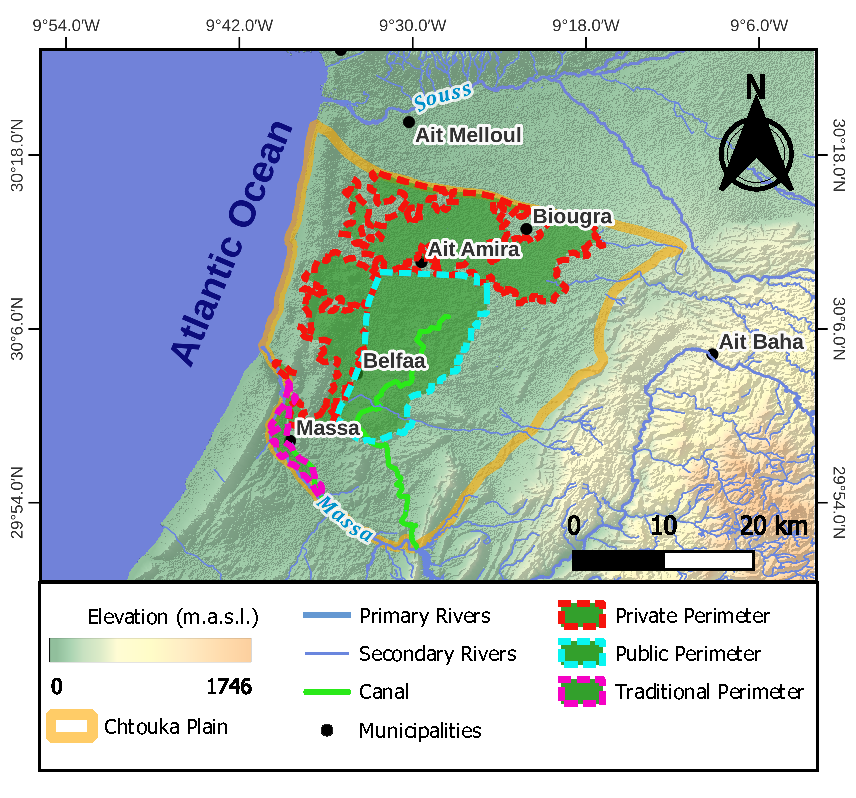
\includegraphics[width=1\textwidth]{./img/Map_ChtoukaOverview.pdf}
    \caption{Map showing the Chtouka plain and its irrigation perimeters. The map is derived from the digital elevation model data of \cite{NASA.SRTM1Arc}.}
    \label{Map-ChtoukaOverview}
\end{figure}

\begin{figure}[p]
    \centering
    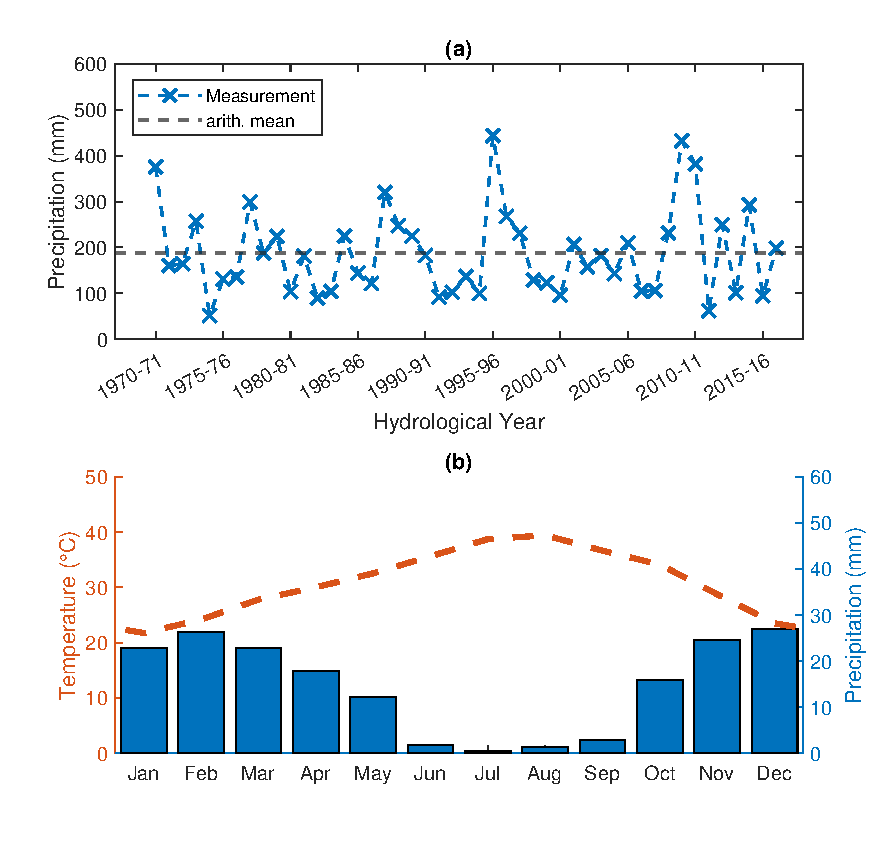
\includegraphics[width=1.0\textwidth]{./img/Fig-PrecNClimateChtouka.pdf}
    \caption{Climatic conditions in the Chtouka-Massa plain. (a): Annual precipitations at the city of Biougra for the period 1970 to 2016. Measurement periods are the respective hydrological years, which range from 1st of September of the denoted year to 31st of August of the following year. The underlying dataset was provided by the ABHSM. (b): Long-term average temperatures and precipitation during a year. The climate chart bases on data for the years 1950-2017 and is derived from the globally gridded monthly time series datasets by \textcite{Matsuura.2018T} and \textcite{Matsuura.2018P}.}
    \label{Fig-ClimateChart}
\end{figure}

Over the years, precipitation show a high variability between years with over $600 \, \textrm{mm} \, \textrm{a}^{-1}$ (three times the long-term average) in humid years and less than $50 \, \textrm{mm} \, \textrm{a}^{-1}$ (a quarter of the long-term average) in dry years. 
Potential evapotranspiration on the other hand lies at approximately $2000 \, \textrm{mm} \, \textrm{a}^{-1}$ in the Souss Massa Basin \parencite{Choukr.2017} and therewith significantly exceeding water supplies through rainfall, as typical for arid and semi-arid climates. 
It may be noted that as basis for yearly measurements the local hydrological year is from 1st of September to 31st of August of the following year. 
Following this convention, in this work this specific hydrological year is always implied, whenever a "year" is referenced. 
For ease of reading however, instead of the full label (e.g. "2021-22") only the first calendar year will be shown in labels ("2021").



\section{Hydrology}
\label{Sec-SouMaHydrology}

In the Souss-Massa Basin, in average $1093 \, \textrm{Mm}^3$ of water are available according to ABHMSM (as cited by \textcite{Choukr.2017}), consisting of $36 \, \%$ surface water and $64 \, \%$ groundwater \parencite{Choukr.2017}. 
Surface water is mainly provided by the two homonymous rivers. 
Depending on the yearly rainfall, surface water potential shows a large variability from year to year (\cite{Choukr.2017}, \cite{ABHSM-HydStats.2022}). 
To regulate the flows of both rivers and ensure a regular supply of water in the Souss-Massa Basin, a total of eight dams have been built in the period from 1972 to 2004 \parencite{Choukr.2017}. 
These dams have a total potential capacity of $730 \, 404 \, \textrm{Mm}^3$. 
Of these, the Youssef Ben Tachfine (YBT) dam which was put into service in 1972 and is functioning since 1974, is the largest with a potential capacity of approximately $300 \,000 \, \textrm{Mm}^3$ \parencite{ABHSM-Dams.2022}. 
It is located in the south-east of the Chtouka plain (Figure \ref{Map-ChtoukaOverview}).

The Souss River originates to the north in the High Atlas mountains where its tributaries form a dense drainage network and to the south in the Anti Atlas where the tributary network is lighter \parencite{Hssaisoune.2017}. 
After confluencing from its different tributaries, the river flows from east to west over $182 \, \textrm{km}$ through the Souss plain, from which it ultimately discharges to the west into the Atlantic Ocean near Agadir (Figure \ref{Map-SoussMassaRegion}). 
Its flow is strongly seasonal, and during rainy years high floods can occur between October and February \parencite{Hssaisoune.2017}.

The Massa River, which forms the southern boundary of the Chtouka plain, originates in the Anti Atlas mountains, from where it flows in western to north-western direction towards the Atlantic Ocean. 
At the southern-most corner of the aquifer it supplies the biggest reservoir of the Souss Massa Basin, the Youssef Ben Tachfine (YBT) dam, which regulates the Massa River on the $36 \, \textrm{km}$ of its course to the Atlantic Ocean. 
Downstream of the dam, the river first flows in a small, steep-sided channel of $5$ to $10 \, \textrm{m}$ width with a rather steep topographic gradient. 
Subsequently when reaching the Massa plain near Ifentar it flows in a wider, meandering channel \parencite{Horn.2021}. 
The Massa River exhibits a high variability following annual and interannual climatic irregularities characterised by brief floodings interrupted by long periods of dryness \parencite{Hssaisoune.2017}.

An irrigation canal originating from the YBT dam supplies water to an agricultural area in the centre of the Chtouka plain (Figure \ref{Map-ChtoukaOverview}), which is called the public irrigation perimeter. 
This area is surrounded to the north and west by the private irrigation perimeter. 
Another channel, originating downstream of the YBT dam supplies the Tassila agricultural area near Massa municipality. 
Furthermore, water from the reservoir is used for drinking water supplies of Tiznit and Ifni.

Overall, the principal water resources of the Souss-Massa Basin are the groundwater and the eight dams \parencite{Hssaisoune.2017}. 
The groundwater reservoir is situated solely below the Souss-Massa plain and therewith only up to $700 \, \textrm{m.a.s.l.}$, as the higher parts are mountainous. 
These mountainous areas form major recharge areas of the aquifer.

Although water supply in the Souss Massa Basin consist of both surface water in the homonymous two rivers and their tributaries as well as groundwater from the aquifer, in the Chtouka area groundwater constitutes the major water source. 
Surface water mostly consists of the Massa River along its southern boundary and the irrigation canal supplied by the YBT dam. 
Following very intense precipitation events, some intermittent wadis flow from the Anti Atlas mountains into the Chtouka plain.

In the Souss Massa Basin, water demand is composed of $12.5 \, \%$ drinking water and water for industrial use, and $86 \, \%$ for agricultural purposes \parencite{Choukr.2017}. 
The water demand is seasonal, as irrigation and tourism are in summer more extensive, while at the same time natural water supply is minimal \parencite{Choukr.2017}. 
In the hydrological year 2018 the YBT dam supplied $51 \,018 \, \textrm{Mm}^3$ for irrigation and $8 \, 208 \, \textrm{Mm}^3$ for drinking purposes \parencite{ABHSM-HydStats.2022}.

In the Souss Massa Basin water exploitation increased significantly in the last decades due to increased irrigated agriculture, tourism and industrial development (\cite{Choukr.2017}, \cite{Hssaisoune.2017}). 
Therefore groundwater levels decreased over the past four decades within a range of $0.5 - 2.5 \, \textrm{m}\, \textrm{a}^{-1}$ due to overpumping \parencite{Choukr.2017} \parencite{Hssaisoune.2017}. 
This led to deterioration of groundwater due to saltwater intrusion in coastal areas and deep well drilling over the past decade \parencite{Choukr.2017}.

For the Chtouka aquifer, the water imbalance between recharge and withdrawal of groundwater evaluated to be $58 \, \textrm{Mm}^3 \, \textrm{a}^{-1}$ in 2007 \parencite{ABHSM-EauSout.2022}. 
Furthermore the quality of the water resources degraded in the course of the last decades due to pollution mainly stemming from domestic, industrial and agricultural wastewaters and fertilisers. 
For example, nitrate concentrations exceed the regulatory threshold value of $50 \, \textrm{mg} \, \ell^{-1}$ for drinking water in $36 \, \%$ of the wells in the Chtouka plain \parencite{Choukr.2017}. 
In the next decades water demand is expected to further increase in the whole region due to population growth, increase in per capita consumption and extension of irrigated agriculture \parencite{Choukr.2017}. 
Simultaneously a decline in water availability is expected due to overpumping of groundwater and lower recharge through rainfalls, which in turn is caused by developing urbanisation and climate change (\cite{Choukr.2017} \cite{Hssaisoune.2017}). 
To tackle these issues, in 2008 the "Plan directeur d'aménagement intégré des ressources en eau (PDAIRE)" was published. 
Besides a revised and itensified management of available water resources and the efficiency enhancement of water consumption, it aims at the exploitation of unconventional water resources such as wastewater reuse and the desalinisation of seawater \parencite{Choukr.2017}.

\section{Economical Structure of the Region}
\label{Sec-SouMaStructure}

Climate conditions in the Souss-Massa Basin provide conditions for a characteristic all-year round growing season \parencite{Hssaisoune.2017}. 
Therefore, the area is extensively used for agricultural production. 
On national level, agriculture has a growing contribution to the Morrocan gross domestic product (GDP), from $7 \, \%$ in 1998-2008 to $17 \, \%$ in 2008-2018 and thus plays a key role in Morocco's economical development \parencite{MarocVert.2021}. 
In this sector the Souss-Massa plain is economically the second most important region in Morocco \parencite{Choukr.2017}. 
The economy of the region is primarily founded on the high-value agricultural production, tourism and fishery. 
Covering more than one fifth of this area the Chtouka plain accounts for a significant portion of the agricultural production of the region \parencite{Choukr.2017}.

On administrative level, the Chtouka plain is part of the Chtouka-Ait Baha province, which reaches to the east past the plain and further into the Anti Atlas mountains. 
In this province a total population of $371 \, 102 \, \textrm{people}$ was counted in 2014, of which $113 \, 531 \, \textrm{people}$ lived in one of the four urban centres (Ait Baha, Biougra, Belfaa, Massa) and the rest in the 18 rural communes \parencite{DRSM.2020}. 
In the period between 2004 and 2014 the population of the province had an average annual growth rate of $2.24 \, \%$ \parencite{DRSM.2020}. 
As shown by these numbers, the Chtouka plain is primarily a rural region.

With a year-round growing season, the Souss Massa Basin accounts besides other products for more than half the production of Moroccan citrus and vegetables \parencite{Hssaisoune.2017}. 
In the Chtouka plain, tomatoes and peppers are cultivated in greenhouses \parencite{DRSM.2020} and furthermore other vegetables and fruits, cereals, fodders, ornamental crops and deciduous trees (Office Regional de Mise en Valeur Agricole de Souss-Massa, as cited by \cite{Malki.2017}). 
Surveys from 2015 identified a total number of 2724 farms covering an area of approximately $24\,800 \, \textrm{ha}$ and which employ more than $40\,000 \, \textrm{people}$ (ABHSMD, 2015, as cited by \cite{Choukr.2017}). 
The majority of these farms are located around Ait Amira, Belfaa, Biougra, Sidi Bibi and Massa (Figure \ref{Map-ChtoukaOverview}). 
Like the whole region of the Souss Massa Basin \parencite{Choukr.2017}, irrigated areas in the Chtouka-Massa plain show an continuous expansion in the past decades.

In the area, three different irrigation practices are being used: flooding, sprinkler and drip irrigation. 
These different irrigation techniques exhibit different water usage efficiencies, with flooding being the least and drip irrigation being the most efficient. 
Simultaneously, these methods require a different technological development and therewith investment of farms, which is why their application highly depends on the economical organisation and situation of the farms \parencite{Choukr.2017}. 
Thus, the implementation of the different techniques varies both spatially and temporally over the agricultural area. 
Due to the problem of overexploitation of water resources (see Section \ref{Sec-SouMaHydrology}), and following the agricultural strategy plan "Plan Maroc Vert" which was adopted in 2008 and its National Irrigation Water Saving Program, efforts have been made to significantly increase the portion of water efficient drip irrigation in the past $15 \, \textrm{years}$ \parencite{MarocVert.2021}. 
For instance, in the northern and north-western private perimeter where structured agri-business farms predominate, an extensive conversion to drip irrigation took place in recent years (ABHSMD, 2015, as cited by \cite{Choukr.2017}). 
At the same time, in the centrally located public perimeter sprinkler irrigation is still the predominant method. 
Furthermore, in these two perimeters cultivation widely takes place in greenhouses. 
At the traditionally farmed Tassila perimeter in the south, along the Massa River, water-intensive flooding is still the major technique. 
The extents of the private perimeter varied over the decades, whereas the public and traditional perimeter remained in constant extents. 
Their respective estimated boundaries for the period 2010-2019 are shown in Figure \ref{Map-ChtoukaOverview}.